%%%%%%%%%%%%%%%%%%%%%%%%%%%%%%%%%%%%%%%%%%%%%%%%%%%%%%%%%%%%%%%%%%%
%TO AVOID FORMATTING ISSUES, COMPILE THIS ONLY AT WWW.OVERLEAF.COM%
%%%%%%%%%%%%%%%%%%%%%%%%%%%%%%%%%%%%%%%%%%%%%%%%%%%%%%%%%%%%%%%%%%%
%AUTHOR: ABHINAV BAKSHI
%CLASS:  BE C 302
%%%%%%%%%%%%%%%%%%%%%%%%%%%%%%%%%%%%%%%%%%%%%%%%%%%%%%%%%%%%%%%%%%%
\documentclass[a4paper,12pt]{article}
\usepackage{graphicx}
%To use this font, you need XeTex or LuaTex, prefer openleaf
\newenvironment{codefont}{\fontfamily{ccr}\selectfont}{\par}

\title{
	\normalfont \normalsize 
	\textsc{Pimpri Chinchwad College of Engineering \\ 
		Computer Laboratory - III} \\
	[10pt] 
	\rule{\linewidth}{0.5pt} \\[6pt] 
	\huge Assignment No - B10 \\
	\rule{\linewidth}{2pt}  \\[10pt]
}
\author{}
\date{\normalsize}


\begin{document}
	\maketitle
	
	%%%%%%%%%%%%%%%%%%%%%%%
	% FOR A NUMBERED LIST
	% \begin{enumerate}
	% \item Your_Item
	% \end{enumerate}
	%%%%%%%%%%%%%%%%%%%%%%%
	% FOR A BULLETED LIST
	% \begin{itemize}
	% \item Your_Item
	% \end{itemize}
	%%%%%%%%%%%%%%%%%%%%%%%
	% TO IMPORT AN IMAGE
	% \includegraphics[width=\textwidth]{name_of_file}
	% \textwidth makes the picture the width of the paragraphs
	%%%%%%%%%%%%%%%%%%%%%%%%%%%%%%
	% TO CREATE A FIGURE WITH A NUMBER AND CAPTION
	% \begin{figure}
	% \includegraphics[width=\textwidth]{image}
	% \caption{Your Caption Goes Here}
	% \label{your_label}
	% \end{figure}
	% REFER TO YOUR FIGURE LATER WITH
	% \ref{your_label}
	% LABELS NEED TO BE ONE WORD
	%%%%%%%%%%%%%%%%%%%%%%%%%%%%%
	% TO ADD CODE
	% \begin{codefont}
	% Some code in "courier" font
	%\end{codefont}
	%%%%%%%%%%%%%%%%%%%%%%%%%%%%%


\section{TITLE : }   Use Business intelligence and analytics tools to recommend the combination of share purchases and sales for maximizing the profit.

\section{MATHEMATICAL MODEL : }

{\rmfamily
	mathematical model is given as below,}


\bigskip

\textrm{S=fs,e,X,Y,Fme,DD,NDD,Mem sharedg}


\bigskip

{\rmfamily
	Where,}

{\rmfamily
	s = Initial State}

{\rmfamily
	e = End State}

{\rmfamily
	X=input
	Datasets of share market.
	
	{\rmfamily
		Y=output
		Bar chart of frequency distribution of share market.}
	
	{\rmfamily
		Fme=Algorithms used (Apriori)}
	
	\textrm{\ for eg.fnextdistance(),estimate(),pathFind()g}
	
	{\rmfamily
		DD=Deterministic Data
		Share market data.
	}
	
	{\rmfamily
		NDD=Non-Deterministic Data.}
	
	{\rmfamily
		Mem-shared=memory shared by the applications.}
	
	
	\bigskip

\section{THEORY : }

Definition: It is a place where shares of pubic listed companies are traded. The primary market is where companies float shares to the general public in an initial public offering (IPO) to raise capital.

Description: Once new securities have been sold in the primary market, they are traded in the secondary market—where one investor buys shares from another investor at the prevailing market price or at whatever price both the buyer and seller agree upon. The secondary market or the stock exchanges are regulated by the regulatory authority. In India, the secondary and primary markets are governed by the Security and Exchange Board of India (SEBI).

A stock exchange facilitates stock brokers to trade company stocks and other securities. A stock may be bought or sold only if it is listed on an exchange. Thus, it is the meeting place of the stock buyers and sellers. India's premier stock exchanges are the Bombay Stock Exchange and the National Stock Exchange.

Conclusion:
Hence we have used business intelligence and analytics tools  KNIME to recommend the combination of share purchases and sales for maximizing the profit.

\begin{itemize} 	
\newpage
\item Input:

Training Data:
 \begin{center}
	\begin{figure}[!htbp]
		\centering
		\fbox{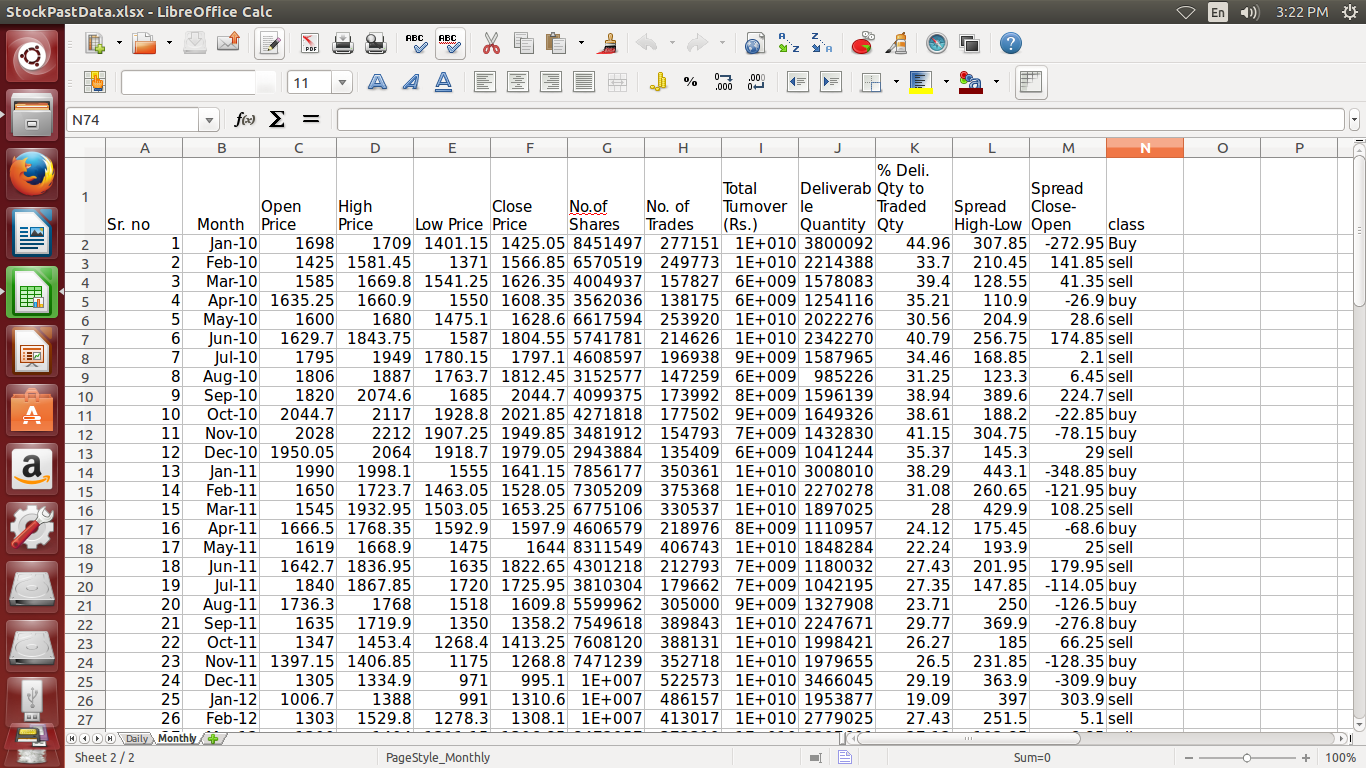
\includegraphics[width=\textwidth]{stock.png}}	
	\end{figure}
\end{center} 

\begin{center}
	\begin{figure}[!htbp]
		\centering
		\fbox{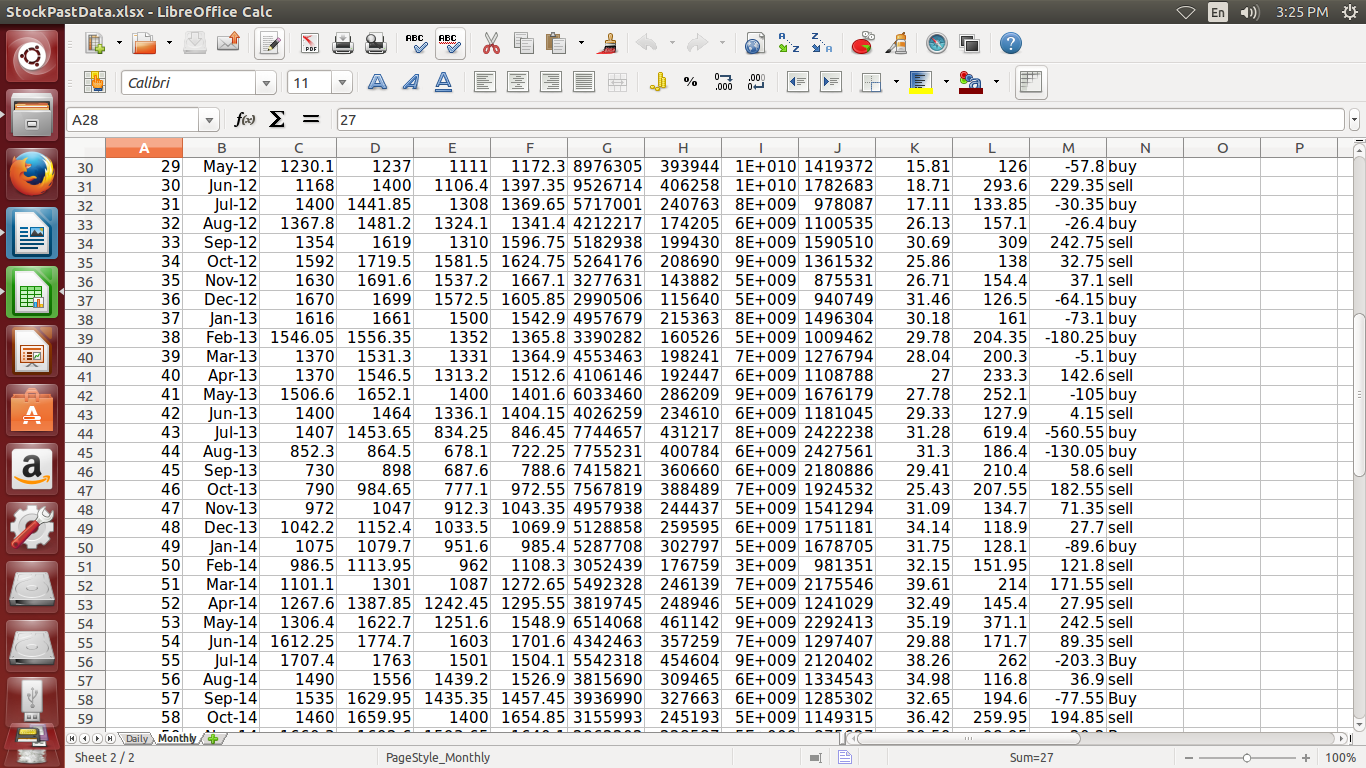
\includegraphics[width=\textwidth]{testing.png}}	
	\end{figure}
\end{center} 

\newpage

\item output

\begin{center}
	\begin{figure}[!htbp]
		\centering
		\fbox{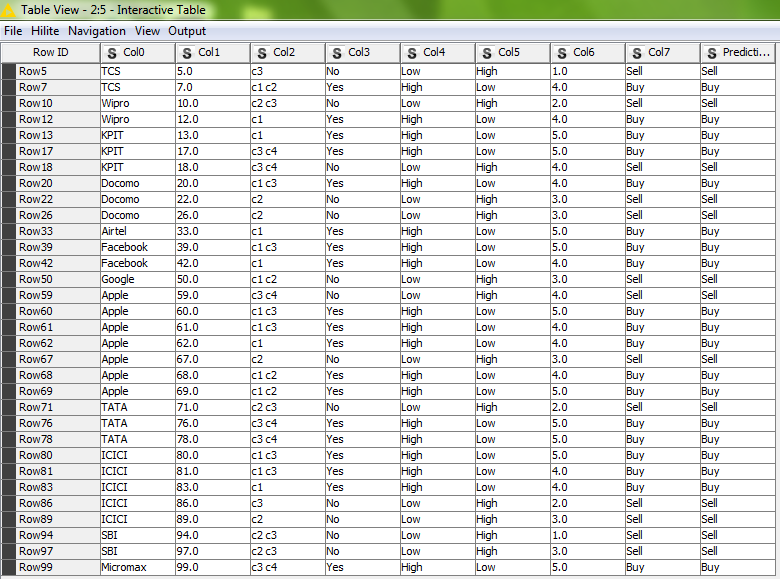
\includegraphics[width=\textwidth]{interactive_output.png}}	
	\end{figure}
\end{center} 

\begin{center}
	\begin{figure}[!htbp]
		\centering
		\fbox{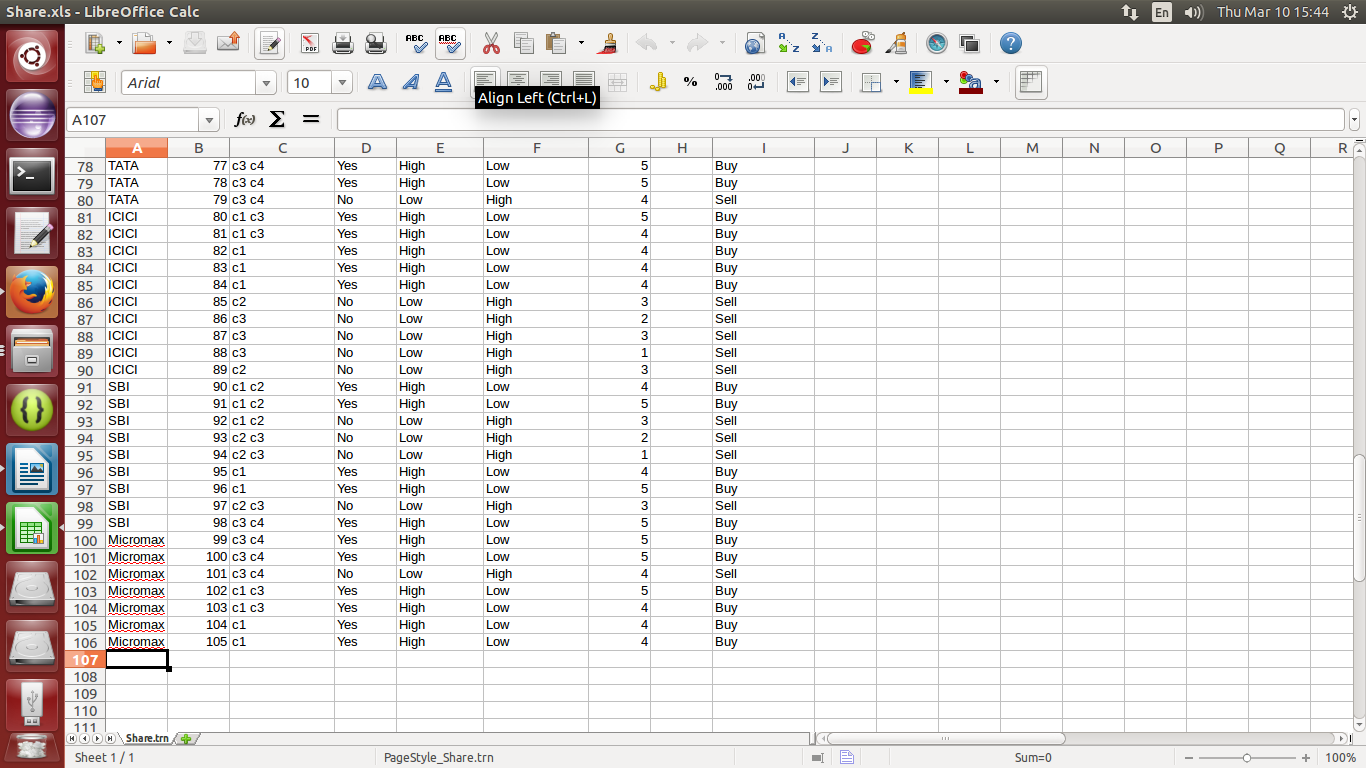
\includegraphics[width=\textwidth]{img1.png}}	
	\end{figure}
\end{center} 
\begin{center}
	\begin{figure}[!htbp]
		\centering
		\fbox{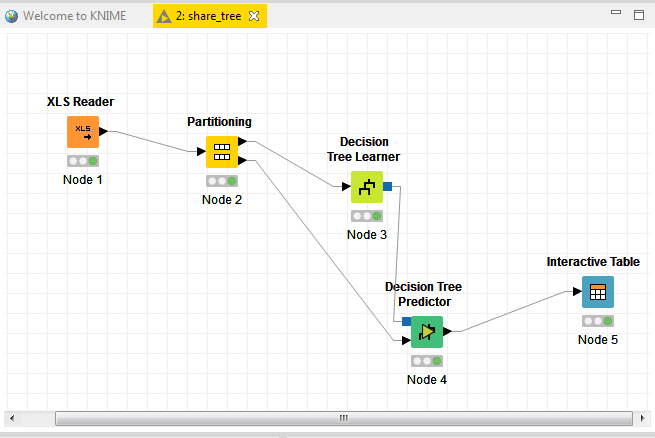
\includegraphics[width=\textwidth]{img2.png}}	
	\end{figure}
\end{center} 
\begin{center}
	\begin{figure}[!htbp]
		\centering
		\fbox{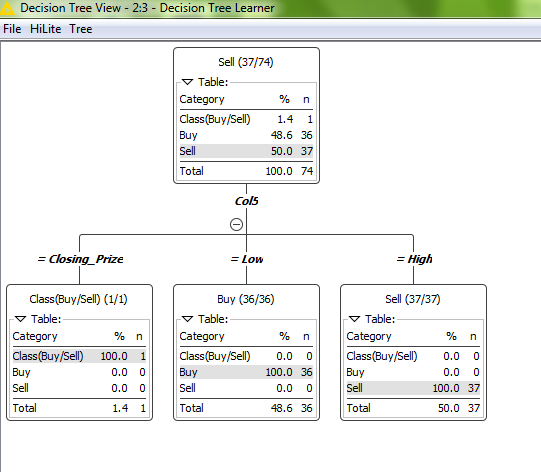
\includegraphics[width=\textwidth]{img3.png}}	
	\end{figure}
\end{center} 

\end{itemize}

\begin{center}
	\newpage	
	\begin{tabular}
		{|c|c|c|c|c|}\hline
		{\bf Roll No.}		&{\bf Name of Student}	&{\bf Date of Performance}  				&{\bf Date of Submission}	&{\bf Sign.}  \\    \hline
		302	& Abhinav Bakshi & 15/12/2015	& 	5/01/2016	&  \\ \hline
	\end{tabular}\\ 
\end{center}
\end{document}
 